%%%%%%%%%%%%%%%%%%%%%%%%%%%%%%%%%%%%%%%%%%%%%%%%%%%
%
%  New template code for TAMU Theses and Dissertations starting Fall 2016.  
%
%
%  Author: Sean Zachary Roberson
%  Version 3.17.09
%  Last Updated: 9/21/2017
%
%%%%%%%%%%%%%%%%%%%%%%%%%%%%%%%%%%%%%%%%%%%%%%%%%%%

%%%%%%%%%%%%%%%%%%%%%%%%%%%%%%%%%%%%%%%%%%%%%%%%%%%%%%%%%%%%%%%%%%%%%%%
%%%                           SECTION II
%%%%%%%%%%%%%%%%%%%%%%%%%%%%%%%%%%%%%%%%%%%%%%%%%%%%%%%%%%%%%%%%%%%%%%


\chapter{METHODS}
\section{Basic Altimeter Test Bed Setup}
In addition to laying out performance standards for radar altimeters, the DO-155 standards~\cite{noauthor_minimum_1974} also specify a basic test setup for verifying an altimeter is functioning properly. Figure~\ref{fig:Basic Testbed} shows the diagram of this test setup. The standards also elaborated on the necessary characteristics of the most critical part of the testbed, the altitude simulator. 

The altitude simulator needed to ''consist of variable and fixed RF attenuators''~\cite{noauthor_minimum_1974}  to simulate the loop loss an altimeter experiences aboard an aircraft (see section 1.6.3). The altitude simulator also needed a length of ''coaxial cables or other suitable delays''~\cite{noauthor_minimum_1974}  to simulate the physical time delay experienced by an altimeter signal between the transmitter and receiver (see section 1.6.2). To complete the test setup, the altitude simulator directed the attenuated and delayed RF energy from the transmitter fed back into the receiver. 
\begin{figure}[ht]
\centering
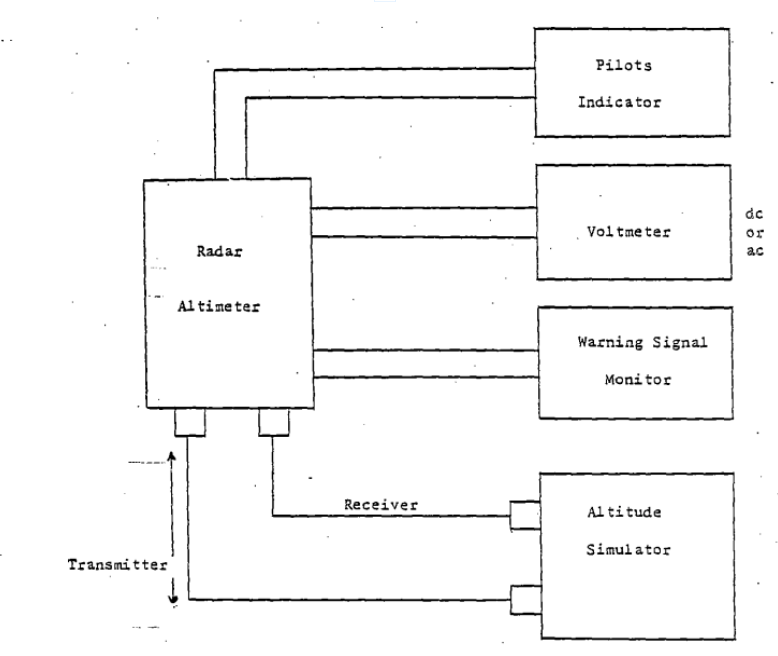
\includegraphics[scale=0.5]{DO-155_Test_Setup.PNG}
\caption[]{Basic Altimeter Test Setup from DO-155~\cite{noauthor_minimum_1974}}

\label{fig:Basic Testbed}

\end{figure}

Additionally, the standards specified that any test equipment must account for cross coupling between transmitting and receiving antennas. DO-155 emphasized that the altitude simulator should achieve the desired altitude within 1\% and the correct attenuation within 2.5dB~\cite{noauthor_minimum_1974}.

\section{Modified Altimeter Test Setup} 
AVSI designed a modified version of the altimeter test setup specified by DO-155, shown in Figure~\ref{fig:Modified Testbed}. The modifications allow the controlled injection of interference into the line after the altimeter signal passes  through the altitude simulator. 

\begin{figure}[ht]
\centering
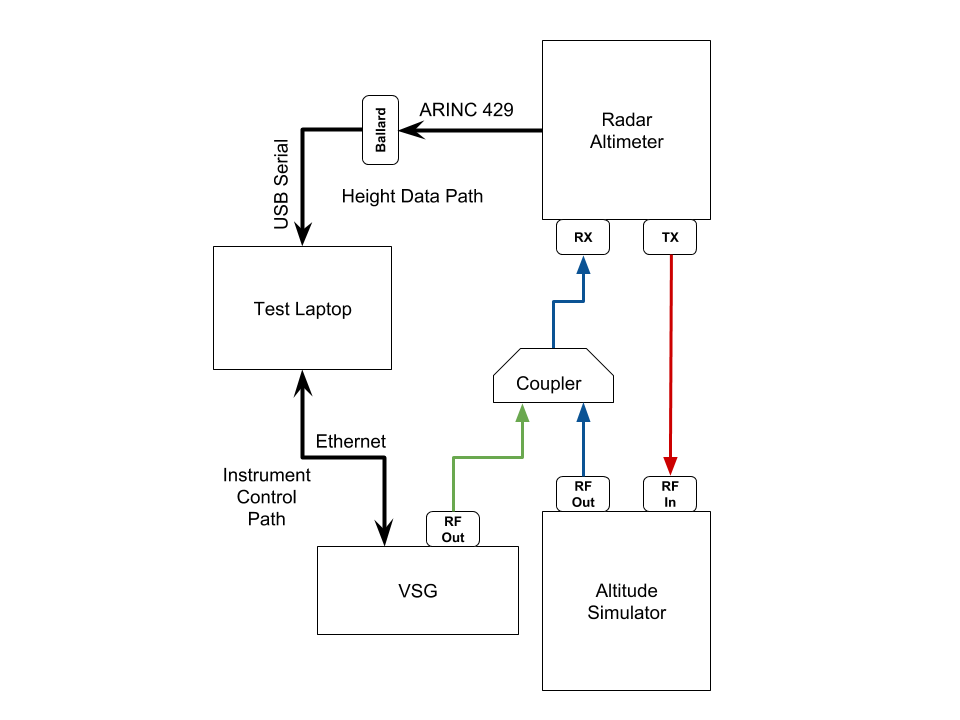
\includegraphics[scale=0.45]{Modified_Test_Setup.png}
\caption[]{Modified Altimeter Test Setup}

\label{fig:Modified Testbed}

\end{figure}
\subsection{Reading the Altimeter Output}
The altimeter outputs labeled height data on a standardized ARINC 429 cable configuration. The modified setup uses a Ballard ARINC device to convert the data from ARINC 429 to USB serial format, providing each data point with a time stamp. On the test laptop, Ballard CoPilot software reads the serial data and provides a display which allows the real time monitoring of all altimeter output and labels. The labels are critical because some data points may be labeled NCD, or No Computed Data, when conditions are insufficient for a reliable height measurement. CoPilot software also allows for the easy export of test data to Microsoft Excel documents for post processing. 
\subsection{Implementing the Altitude Simulator}
\subsubsection{Time Delay}
Different test altitudes required the use of different methods of delaying the RF energy output by the altimeters. For higher altitude tests, spools of fiber optic cables created a time delay. The RF output from the altimeter transmitter was fed by coax connection to the fiber optic transceiver, which could either pass the signal to a single fiber optic spool or a series of cascaded spools to achieve a desired height. This setup contained optical spools of 500, 1000, 2000, and 4500 feet, each of which could be used individually or in conjunction with any or all of the other spools to implement a delay.

 The optical transceiver and cascaded spools also contribute an attenuation to the loop loss which varies based on the number of spools cascaded. A single spool setup has an attenuation verified experimentally to be 29dB, with an additional 2dB loss added for each additional cascaded spool.

Later tests would modify this delay setup to test an altimeter in takeoff and landing scenarios. The much lower height in these scenarios meant that a spool of coax could be used tor the delay instead of fiber optic cables. Two coax spools provided a height of 40 ft and 95 ft for testing these scenarios, with a 6dB and 36dB attenuation contributed to the loop loss respectively.  

\subsubsection{Achieving Standard Loop Losses}
DO-155 specifies loop loss for various heights and antenna types. For these tests, the loop loss used for each height is listed in Table~\ref{tab:loop loss} To achieve the Loop Losses specified by DO-155 standards for each height, the attenuation inherent in the delay method used for each height must be taken into account. Once the attenuation from the delay line is subtracted from the loop loss, 10, 20 and 30dB Pasternack fixed attenuators are inserted into the setup to get within 10dB of the desired loop loss. These are located within the setup in part to protect the fiber optic transceiver from damage.  Finally, a step attenuator capable of 1 to 11 dB is used to achieve the desired loop loss with a 1 dB precision. 

\begin{table}[]
\centering
\begin{tabular}{|c|c|}
\hline
\textbf{Height} & \textbf{Loop Loss} \\ \hline
40ft            & 76 dB              \\ \hline
95ft            & 84 dB              \\ \hline
500ft           & 100 dB             \\ \hline
1500ft          & 109 dB             \\ \hline
3000ft          & 116 dB             \\ \hline
5000ft          & 120 dB             \\ \hline
8000ft          & 124 dB             \\ \hline
\end{tabular}
\caption{DO-155 Loop Losses}
\label{tab:loop loss}
\end{table}

\subsection{Generating Interference Signals}
A Rhode and Schwarz SMU200A Vector Signal Generator (VSG) is used to generate simulated WAIC signals of varying modulation types, bandwidths and power levels. The VSG has a SCPI interface which allows an external computer to control any functionality on the instrument through commands sent over either a serial or an Ethernet connection. 

The VSG allows full control of an RF generator along with two baseband generators. The RF generator gives the user control of RF carrier frequency as well as the output power level of the carrier in dBm. The baseband generators allow the modulation of two potentially unique waveforms onto the carrier wave, with a possible offset frequency from the center. 

\section{Python Test Software}


Python code written by the author pieces together the various parts of this setup into a complete test bench. Different Python scripts handle different functions necessary to the test bench. These include:

\begin{itemize}
\item Creating a database to transfer data between different Python Scripts
\item Interface with the VSG to generate interference signals
\item Parse the CoPilot log
\item Mapping time stamped height measurements to time stamped interference signals
\item Plotting and analyzing the results
\end{itemize}

\begin{figure}[ht]
\centering
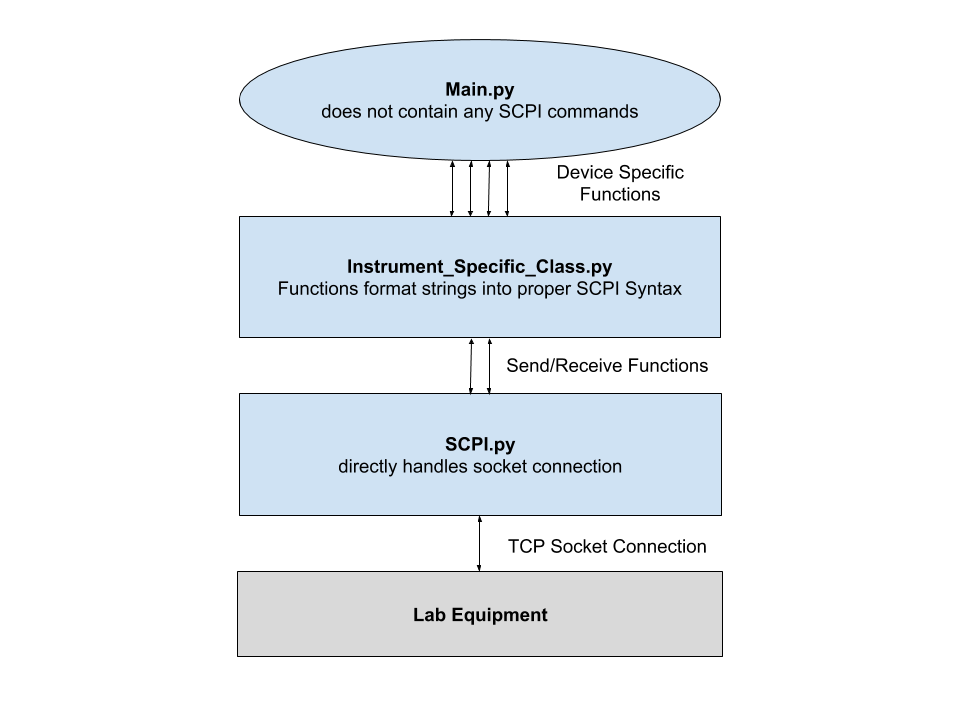
\includegraphics[scale=0.45]{SCPI_Class_Hierarchy.png}
\caption[]{SCPI Class Hierarchy}

\label{fig:SCPI}

\end{figure}
The software uses Standard Commands for Programmable Instruments or SCPI to control the vector signal generator. In this test bed, the SCPI instructions are processed through an object-oriented hierarchy shown in Figure~\ref{fig:SCPI}. The superclass, $SCPI$ interfaces directly with all lab equipment. The subclass, called \textit{RS\_Signal\_Generator} in this implementation, contains python functions associated with all instrument specific commands. The helper functions from $SCPI$ send and receive communication with the instrument. Finally, the main loop exists at the highest level, which times the calls of different instrument commands and creates a database to store them. 

\subsection{Test Main Loop}
The highest level of this design is the test main loop. The test main loop creates the SQLite database which stores all important information for easy transfer between the different python scripts necessary for the test bed. This program also contains variables for various test parameters, which are stored in an SQLite database for easy reference and sometimes directly control the sequence of a test. Finally, this program loops through the sequence interference signals specified by the various test parameters, and sends the commands to the VSG to generate them. The commands sent to the VSG are time stamped as precisely as possible, and recorded in the \textit{Generated Signals} table in the database. 


Certain test parameters are stored for reference or calculation but do not directly affect the sequence of interference signals to be generated. These include the altimeter make and model, the nominal height of the test setup, the loss experienced by interference signals traveling to the altimeter RX, and the loop loss used in the setup. Other parameters directly control the sequence of the test, including interference on and off times, power levels to be used, modulation formats to be tested, and RF carrier frequencies to be used. 

\subsubsection{Nominal Height vs Correct Height}
\textit{Nominal height} is the term used to refer to the height of the test setup. For example, the smallest spool of fiber optic cable is 500ft long, so the test setup using only this spool in the altitude simulator has a \textit{nominal height} of 500ft.  However, the measured height in a particular setup will typically differ from the nominal height by a small amount.  This small offset varies between the different altimeters under test. The difference between measured height and the nominal height of the setup can be attributed in part to the extra cabling going to and from the altitude simulator, but primarily is a result of different calibration settings for each altimeter. 

The calibration procedure is an important part of installing an altimeter onto an aircraft. When an aircraft is on the ground, the TX and RX antennas used by the altimeter are naturally several feet off the ground, in line with the airframe. To compensate for the varying heights of airframes, avionics manufacturers developed a calibration procedure so that each altimeter could be programmed upon installation to output an altitude of 0ft when the plane is on the ground. Because these tests are only concerned with \textit{height error}, rather than the most precise height measurement possible in the setup, this calibration is not corrected for in test procedures. Instead, a variable called \textit{correct\_height} is calculated in post processing as the median altitude with no interference. Any height error attributable to interference is measured as a distortion from this correct height.

\subsubsection{Sequence Control}
The primary purpose of the test main loop is to subject an altimeter to various modulation formats, gradually stepping up the power of each until the altitude readings from an altimeter are distorted or broken. The main loop determines the type of modulation, power level, and timing, and as each signal is turned on or off by the VSG, stores the parameters for the signal in the \textit{Interference Signals} table for use in post processing, an example of which is shown in Table ~\ref{tab:Interference}. Each unique modulation format and power combination will have two entries in the \textit{Interference Signals} table, corresponding to the RF ON and RF OFF states of the VSG.  

A variety of parameters controls the progression of different interference signals.  The \textit{interference\_duration} and \textit{signal\_off\_duration}, define the length of time the altimeter will be subjected to a particular interference signal, as well as the length of time the altimeter will have to recover from any error caused by the previous signal. Throughout the main loop, each signal's Start Time and End time is calculated using interference duration variables.  



The next variable which is important to the progression of a test is a list called \textit{modulation\_formats}, which contains strings corresponding to the different modulations the VSG will generate. MSK and OFDM signals of varying bandwidths will be listed here. Each string in the modulation formats list will be passed to a helper function called \textit{choose\_carrier\_frequency\(\)}, which gives the option for different modulation formats to be put on different carriers, as well as for carrier 
\begin{table}[]
\begin{tabular}{@{}lllllll@{}}
\toprule
ID & Altimeter   & Start Time          & End Time            & Modulation & Power dBm & RF State \\ \midrule
1  & Altimeter A & 2017-06-11 19:23:06 & 2017-06-11 19:23:07 & MSK        & -10       & OFF      \\
2  & Altimeter A & 2017-06-11 19:23:07 & 2017-06-11 19:23:08 & MSK        & -10       & ON       \\ \bottomrule
\end{tabular}
\caption{Example Interference Signals Table}
\label{tab:Interference}
\end{table}
 \textit{power\_min}, \textit{power\_max}, and \textit{power\_step} 


\subsubsection{Precision of Timing Commands}



%\subsection{VSG Class}
%\subsection{SCPI Class}
%\subsection{Post - Processing}
%\subsubsection{Parsing The Copilot Log}
%\subsubsection{Mapping Interference Signals to Copilot Data}
%\subsubsection{Plotting the Data}
%
%\section{Setup for WAIC plus Altimeter Interference}
%
%\subsection{Calibrating the VCOs}
%
%\section{Setup for Testing Wider Bandwidth Interference}
%
%\subsection{Handling Multiple Vector Signal Generators}
